\chapter{String Theory and M-Theory}

This chapter follows Leonard Susskind's lecture as a deliberate return to T-duality. We are not going back merely to repeat the slogan that a small compact circle can be traded for a large one. The lecture goes back because that statement has a mathematical core, because that core becomes sharper when written on the worldsheet, and because once one pushes it onto open strings it forces entirely new objects into the theory. The transcript is the primary guide throughout; the selected blackboard frames preserved by LazyingArt LLC and Video2Book are kept where they stabilize an equation, a diagram, or the grouping of fields on the board.

\section{Compactification, Closed Strings, and the Meaning of \(\sigma\)}

The lecture begins by rebuilding the setting from the ground up. We imagine toroidal compactification, since circles, two-tori, and higher-dimensional tori are the simplest compact spaces to analyze. Then, to make the discussion concrete, we strip the geometry down to one large spatial direction \(x\) and one compact direction \(y\). Time is present but suppressed from the picture.

To remain close to the lecture, we write the compact identification as
\begin{equation}
y \sim y+r,
\end{equation}
where \(r\) is the size of the compact cycle in the lecturer's loose notation. In stricter conventions one would distinguish radius from circumference and keep track of the accompanying \(2\pi\) factors. Here we do the opposite: we regularize the notation enough to make the formulas coherent, but we stay as close as possible to the lecture's units and pacing.

The objects of interest at first are closed oriented strings. Their embedding coordinates are functions of worldsheet time \(\tau\) and worldsheet position \(\sigma\),
\begin{equation}
x=x(\tau,\sigma), \qquad y=y(\tau,\sigma), \qquad \sigma\sim \sigma+2\pi.
\end{equation}
The strings are closed because they have no endpoints, and they are oriented because there is an intrinsic sense in which one can go around them one way rather than the other. Reversing every orientation everywhere would give the same theory; what matters is the relative comparison between one string and another.

This orientation is not decorative. It constrains the basic process of string theory, namely splitting and joining. When strings split or join, the arrows that record the orientation must remain continuous. That is already the first hint that topological information can survive dynamical processes.

\subsection{Question \& Answer}

\paragraph{Question.} Is \(\sigma\) the same thing as going around the compact direction?

\paragraph{Answer.} No. This is the first conceptual obstacle in the lecture, and it is worth resolving carefully because the whole later discussion depends on it. The coordinate \(\sigma\) is only a label for points along the string. It runs once around every closed string, wound or unwound. One may think of Susskind's rubber-band analogy: the molecules of a rubber band can be named in order as one goes around it, but that naming has nothing to do with whether the rubber band is wrapped around one's wrist.

Winding is therefore not a statement about \(\sigma\) by itself. It is a statement about the map \(\sigma \mapsto y(\tau,\sigma)\). The parameter \(\sigma\) always goes once around the string itself. The image of the string in real space may go around the compact \(y\)-direction zero times, once, many times, or in the opposite orientation. Those are different physical statements, and later we will need them to remain sharply distinct.

\section{Winding, Orientation, and Conserved Topology}

Once \(\sigma\) has been separated from real space, the lecture turns to wound and unwound strings. An unwound closed string is just a closed loop moving in a space with one compact coordinate. A wound string, by contrast, wraps the compact direction. Because the string is oriented, there are two elementary one-fold windings, opposite to each other.

The lecture does not define winding number abstractly and then move on. It earns it through pictures of what can happen. That order matters. We first watch strings join and split, and only then do we read off the conserved quantity.

Take two strings wound in opposite directions. The orientation rule allows them to reconnect into a configuration that can be topologically deformed into a single unwound string. In that sense
\begin{equation}
(+1)+(-1)=0.
\end{equation}
Now take two strings wound in the same direction. They can still reconnect, but they do not unwind. The result still carries total winding
\begin{equation}
(+1)+(+1)=2.
\end{equation}
The number of connected components may change, but the total winding does not.

\begin{figure}[htbp]
\centering
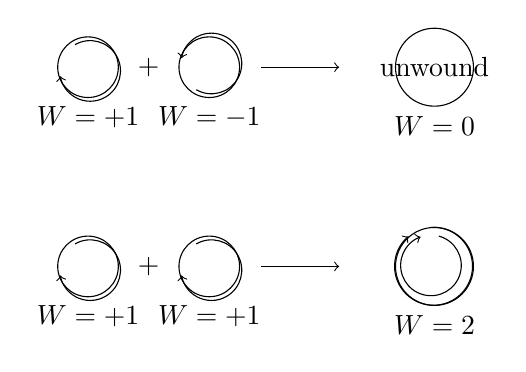
\begin{tikzpicture}[x=1.1cm,y=1.1cm]
\draw (0,1.3) circle (0.35);
\draw[->] (-0.15,1.56) arc (120:-170:0.35);
\node at (0,0.72) {$W=+1$};

\draw (1.4,1.3) circle (0.35);
\draw[->] (1.25,1.04) arc (-120:170:0.35);
\node at (1.4,0.72) {$W=-1$};

\node at (0.7,1.3) {$+$};
\draw[->] (2.0,1.3) -- (2.9,1.3);

\draw (4.0,1.3) circle (0.45);
\node at (4.0,1.3) {unwound};
\node at (4.0,0.62) {$W=0$};

\draw (0,-1.0) circle (0.35);
\draw[->] (-0.15,-0.74) arc (120:-170:0.35);
\node at (0,-1.58) {$W=+1$};

\draw (1.4,-1.0) circle (0.35);
\draw[->] (1.25,-0.74) arc (120:-170:0.35);
\node at (1.4,-1.58) {$W=+1$};

\node at (0.7,-1.0) {$+$};
\draw[->] (2.0,-1.0) -- (2.9,-1.0);

\draw (4.0,-1.0) circle (0.45);
\draw[->] (3.95,-0.55) arc (95:-230:0.45);
\draw[->] (4.05,-0.65) arc (75:-250:0.35);
\node at (4.0,-1.68) {$W=2$};
\end{tikzpicture}
\caption{The two topological moves emphasized in the lecture. Opposite windings can reconnect to an unwound configuration; same-sign windings can reconnect, but the total winding remains nonzero.}
\end{figure}

This is the conservative core of the discussion. A total winding of \(100\) can be distributed in many ways: one string wound \(100\) times, two strings wound \(50\) times each, or a hundred singly wound strings. The lecture insists on this point because it makes winding feel like charge. The carriers may reorganize themselves, but the conserved quantity remains.

So we introduce a total winding number \(W\). Positive and negative windings are distinguished by orientation, and \(W\) is additive under the allowed splitting and joining processes. We do not yet need a formal integral expression for it. For the moment it is enough to know what it does.

\section{Momentum Modes, Winding Modes, and the Closed-String Form of T-Duality}

At this stage the lecture pivots. Up to now winding has been a conserved topology. That alone does not yet give T-duality. To get duality we need the spectrum.

An unwound closed string can move in the compact direction, and because that direction is periodic the compact momentum is quantized:
\begin{equation}
p_y \sim \frac{n}{r}, \qquad E_{\text{mom}} \sim \frac{n}{r},
\end{equation}
with \(n\in\mathbb{Z}\). The lecturer treats an unwound string here as a tiny particle and emphasizes that, in the chosen units, the compact contribution to the energy is of the same scale as the compact momentum itself.

A wound string carries energy differently. String tension is energy per unit length; in the lecture one works in units where that tension is set to \(1\). A string wound \(w\) times around the compact cycle therefore carries energy
\begin{equation}
E_{\text{wind}} \sim w\,r.
\end{equation}

Now the comparison becomes immediate. If \(r\ll 1\), then the momentum spacing is large while the winding spacing is small:
\begin{equation}
\Delta E_{\text{mom}} \sim \frac{1}{r}, \qquad
\Delta E_{\text{wind}} \sim r.
\end{equation}
If \(r\gg 1\), the situation reverses:
\begin{equation}
\Delta E_{\text{mom}} \sim \frac{1}{r}, \qquad
\Delta E_{\text{wind}} \sim r,
\end{equation}
but now it is the momentum sector that is light and the winding sector that is heavy. The two descriptions exchange roles.

\begin{figure}[htbp]
\centering
\begin{tikzpicture}[x=0.9cm,y=0.65cm]
\draw[->] (0,0) -- (0,7.2);
\node at (0,7.8) {$r\ll 1$};
\node[rotate=90] at (-0.9,3.6) {$E$};
\node at (1.0,6.7) {momentum};
\foreach \yy/\lab in {0/0,2.8/1,5.6/2} {
  \draw (-0.25,\yy) -- (0.25,\yy);
  \node[right] at (0.3,\yy) {$n=\lab$};
}
\draw[->] (4,0) -- (4,7.2);
\node at (5.0,6.7) {winding};
\foreach \yy/\lab in {0/0,0.7/1,1.4/2} {
  \draw (3.75,\yy) -- (4.25,\yy);
  \node[right] at (4.3,\yy) {$w=\lab$};
}

\draw[->] (8,0) -- (8,7.2);
\node at (8,7.8) {$r\gg 1$};
\node at (9.1,6.7) {momentum};
\foreach \yy/\lab in {0/0,0.7/1,1.4/2} {
  \draw (7.75,\yy) -- (8.25,\yy);
  \node[right] at (8.3,\yy) {$n=\lab$};
}
\draw[->] (12,0) -- (12,7.2);
\node at (13.0,6.7) {winding};
\foreach \yy/\lab in {0/0,2.8/1,5.6/2} {
  \draw (11.75,\yy) -- (12.25,\yy);
  \node[right] at (12.3,\yy) {$w=\lab$};
}
\end{tikzpicture}
\caption{The schematic level spacings described in the lecture. For small \(r\), momentum modes are heavy and winding modes are light; for large \(r\), the roles reverse.}
\end{figure}

This is where the lecture asks the operational question. Suppose all we can measure is the compact contribution to the energy. How would we know whether we are in a theory with a very small compactification radius and light winding modes, or in a theory with a very large compactification radius and light momentum modes? From the spectrum alone, we would not know. The remarkable claim is stronger still: in string theory the equivalence survives all the way to scattering processes. So T-duality is not just a suggestive comparison of energy levels; it is an exact equivalence between two descriptions of the same physics.

At the spectral level the exchange is
\begin{equation}
n \leftrightarrow w, \qquad r \leftrightarrow \frac{1}{r}.
\end{equation}
In the lecture normalization there is a special self-dual point,
\begin{equation}
r=1,
\end{equation}
where the two descriptions literally meet.

But Susskind now wants a sharper formulation. Momentum and winding should each be written as an integral over the string. The total compact momentum is the sum of the momenta of all the little bits of string. Up to the lecture's suppressed normalization factors,
\begin{equation}
P_y \propto \int d\sigma\,\frac{\partial y}{\partial \tau}.
\end{equation}
The corresponding winding expression is visible on the board and can be cleaned up as
\begin{equation}
W=\frac{1}{r}\int d\sigma\,\frac{\partial y}{\partial \sigma}.
\end{equation}
The lower line is directly legible in the lecture frame; the upper line is only partially legible, so it is better to reconstruct the momentum formula from the transcript than to pretend that every factor can be read from the pixels.

\begin{figure}[htbp]
\centering

\includegraphics[width=0.72\textwidth]{lecture_10_figure_03.png}
\caption{Momentum and winding integrals on the board. The lower line is directly legible; the upper line fixes the structure of the momentum integral but not its full normalization.}
\end{figure}

Cleanly written, the pair of worldsheet formulas is
\begin{align}
P_y &\propto \int d\sigma\,\frac{\partial y}{\partial \tau},\\
W &= \frac{1}{r}\int d\sigma\,\frac{\partial y}{\partial \sigma}.
\end{align}

To make the winding formula concrete, the lecture specializes to the simplest once-wound embedding. Here one adopts the lecture's normalization, in which common \(2\pi\) factors are suppressed and \(\sigma\) is measured in units of one circuit. In that normalization one may write schematically
\begin{equation}
\sigma \sim \frac{y}{r},
\end{equation}
so that
\begin{equation}
\frac{d\sigma}{dy}=\frac{1}{r}.
\end{equation}
This is not meant as a textbook normalization identity; it is the lecture's way of saying that one trip around the string corresponds to one trip around the compact direction.

\begin{figure}[htbp]
\centering
\begin{tikzpicture}[x=1cm,y=1cm]
\draw (0,0) ellipse (1,0.35);
\draw (-1,0) -- (-1,3);
\draw (1,0) -- (1,3);
\draw (0,3) ellipse (1,0.35);
\draw[->] (-1.7,0.2) -- (-1.7,1.8) node[left] {$y$};
\draw[->] (-0.7,-0.6) -- (0.8,-0.6) node[right] {$x$};
\draw[thick] (0.4,3.2) .. controls (1.0,2.4) and (-1.0,1.9) .. (-0.4,1.3)
            .. controls (0.9,0.7) and (-0.2,0.2) .. (0.4,-0.2);
\draw[->] (0.12,2.52) -- (0.42,2.28);
\node[right] at (0.55,2.45) {$\sigma$ increases};
\node at (3.5,1.55) {$y(\sigma+2\pi)=y(\sigma)+r$};
\end{tikzpicture}
\caption{A once-wound embedding. The parameter \(\sigma\) still labels the string; winding means that the embedding \(y(\sigma)\) shifts by one compact period as \(\sigma\) goes once around the closed loop.}
\end{figure}

\paragraph{Worked derivation.} With the lecture's normalization understood, the winding integral becomes transparent.
\begin{enumerate}
\item As \(\sigma\) goes once around the closed string, the embedding \(y(\sigma)\) goes around the compact direction \(w\) times.
\item Therefore the total change of \(y\) over one circuit is
\begin{equation}
\Delta y = w\,r.
\end{equation}
\item Hence
\begin{equation}
W=\frac{1}{r}\int d\sigma\,\frac{\partial y}{\partial \sigma}
 =\frac{1}{r}\,\Delta y
 =\frac{1}{r}(w\,r)
 =w.
\end{equation}
\end{enumerate}
So the integral really does count winding.

\subsection{Question \& Answer}

\paragraph{Question.} How can an integral of a derivative measure winding instead of vanishing?

\paragraph{Answer.} Because the quantity being differentiated is not single-valued in the ordinary way. The label \(\sigma\) returns to itself after one circuit, but the embedded coordinate \(y(\sigma)\) returns only modulo the compact identification. In the lecture this is said loosely as ``\(y\) changes by \(2\pi\).'' In the present normalization the clean statement is that \(y\) changes by \(w\,r\). Therefore
\begin{equation}
\int d\sigma\,\frac{\partial y}{\partial \sigma}=\Delta y=w\,r,
\end{equation}
and dividing by \(r\) gives the winding number. The usual argument that the integral of a derivative vanishes is the wrong argument here.

This is the point where the lecture upgrades T-duality from a spectral curiosity to a worldsheet statement:
\begin{equation}
n \leftrightarrow w, \qquad
r \leftrightarrow \frac{1}{r}, \qquad
\frac{\partial y}{\partial \tau} \leftrightarrow \frac{\partial y}{\partial \sigma}.
\end{equation}

\section{Worldsheet Derivatives and the Two Charge Sectors}

The lecture does not move from here directly to D-branes. There is a second pivot. Once momentum and winding have been written as worldsheet integrals, they begin to look less like bookkeeping devices and more like charges.

Susskind even pauses over a natural objection: why should wound strings occur at all? The answer is the same kind of answer one gives for charged particles in quantum field theory. A string does not ``want'' anything. But high-energy collisions can stretch strings, the strings can reconnect, and oppositely wound pairs can be produced and then separate. In that sense winding states are as unavoidable as electron-positron pairs once the dynamics allows them.

So momentum and winding behave as two charge sectors. Opposite charges attract and like charges repel. The lecture first says this for compact momentum, then says it again for winding. The task is now to identify the corresponding fields.

For momentum, the answer comes from five-dimensional gravity. Let \(G_{MN}\) be the five-dimensional metric, with \(M,N\) running over the ordinary spacetime directions together with the compact fifth direction. Then
\begin{equation}
G_{MN}\longrightarrow \{G_{\mu\nu},\,G_{\mu 5},\,G_{55}\}.
\end{equation}
The interpretation is immediate:
\begin{align}
G_{\mu\nu} &\quad \text{is the ordinary four-dimensional metric},\\
G_{\mu 5} &\quad \text{is a four-dimensional vector field},\\
G_{55} &\quad \text{is a scalar modulus controlling the size of the compact direction}.
\end{align}
On the board one sees this precisely as the grouping
\begin{align}
g_{\mu 5} &\mapsto A_\mu,\\
g_{55} &\mapsto \Phi.
\end{align}
In the prose below we write the scalar as \(\phi\), while keeping in mind that the board itself uses a capital \(\Phi\).

\begin{figure}[htbp]
\centering

\includegraphics[width=0.72\textwidth]{lecture_10_figure_04.png}
\caption{Five-dimensional metric components and their four-dimensional descendants. The board emphasizes the mixed component \(g_{\mu5}\) as a vector and \(g_{55}\) as a scalar.}
\end{figure}

Why is \(G_{\mu 5}\) the relevant analog of the electromagnetic potential? Because mixed metric components are sourced by momentum flow in the fifth direction. The compact momentum quantum number is therefore read in the reduced description as an electric-like charge for \(A_\mu\). That is the lecture's Kaluza--Klein reading of the first charge sector.

The second charge sector, winding, needs another field. Here the lecture briefly returns to the closed-string spectrum. The first level-matched massless excitation has one left-moving and one right-moving oscillator,
\begin{equation}
a^i_{1,L}a^j_{1,R}|0\rangle.
\end{equation}
If one of the indices is the compact direction \(5\), then one obtains vector-like states. At the level of schematic oscillator bookkeeping, one may write
\begin{equation}
a^\mu_{1,L}a^5_{1,R}|0\rangle \pm a^5_{1,L}a^\mu_{1,R}|0\rangle.
\end{equation}
One linear combination belongs to the metric sector and produces the momentum-coupled vector \(G_{\mu5}\). The other belongs to the Kalb--Ramond sector and produces a second photon-like field \(B_{\mu5}\), which couples to winding number.

Thus by the end of the closed-string analysis T-duality has been sharpened once more. It is not only
\begin{equation}
n \leftrightarrow w, \qquad
r \leftrightarrow \frac{1}{r}, \qquad
\frac{\partial y}{\partial \tau} \leftrightarrow \frac{\partial y}{\partial \sigma},
\end{equation}
but also, at the level of the corresponding vector fields,
\begin{equation}
G_{\mu5}\leftrightarrow B_{\mu5}.
\end{equation}
The lecture has therefore climbed from topology to spectra, from spectra to worldsheet derivatives, and from worldsheet derivatives to spacetime fields.

\section{Open Strings and the T-Duality Puzzle}

After the break the lecture explicitly resets the story. We now know what T-duality means for closed strings, and we know that the exchange \(\partial_\tau y \leftrightarrow \partial_\sigma y\) is exact. But open strings do not have stable winding number in the closed-string sense. So what can T-duality possibly mean for them?

The lecture begins with the ordinary open-string boundary condition. At the endpoint there may be no net tension; otherwise the endpoint would experience infinite acceleration in the continuum limit. In the toy geometry this gives Neumann boundary conditions
\begin{equation}
\left.\frac{\partial x}{\partial \sigma}\right|_{\partial\Sigma}=0,
\qquad
\left.\frac{\partial y}{\partial \sigma}\right|_{\partial\Sigma}=0.
\end{equation}
One can phrase this almost mechanically: if the endpoint is free, the spatial derivative along the string must vanish there. The lecture also notes the alternative possibility. If someone were holding the endpoint in place and applying an external force, one could have a different boundary condition. That observation will matter in a moment.

\begin{figure}[htbp]
\centering

\includegraphics[width=0.72\textwidth]{lecture_10_figure_05.png}
\caption{The cylinder sketch used for the open-string discussion, together with the partially written boundary condition. The terminal \(0\) comes from the lecture itself rather than from the frozen board state.}
\end{figure}

The crucial point is that T-duality acts only on the compact direction. The long coordinate \(x\) is left alone. Only \(y\) is dualized, so the relevant part of the rule is
\begin{equation}
\frac{\partial y}{\partial \sigma}\leftrightarrow \frac{\partial y}{\partial \tau}.
\end{equation}
If we apply that rule to the open-string endpoint, then the Neumann condition becomes
\begin{equation}
\left.\frac{\partial y}{\partial \sigma}\right|_{\partial\Sigma}=0
\quad \xrightarrow{\,T\,} \quad
\left.\frac{\partial y}{\partial \tau}\right|_{\partial\Sigma}=0.
\end{equation}

\begin{figure}[htbp]
\centering
\begin{tikzpicture}[x=1cm,y=1cm]
\draw (0,0) ellipse (1,0.35);
\draw (-1,0) -- (-1,2.8);
\draw (1,0) -- (1,2.8);
\draw (0,2.8) ellipse (1,0.35);
\draw[->] (-0.7,-0.6) -- (0.8,-0.6) node[right] {$x$};
\draw[->] (-1.6,0.2) -- (-1.6,1.5) node[left] {$y$};
\draw[thick] (-0.3,2.2) .. controls (0.6,1.8) and (-0.2,1.0) .. (0.6,0.5);
\fill (-0.3,2.2) circle (0.05);
\fill (0.6,0.5) circle (0.05);

\node at (3.8,1.5) {$\left.\partial_\sigma y\right|_{\partial\Sigma}=0$};
\node at (3.8,0.9) {$\downarrow\ T$};
\node at (3.8,0.3) {$\left.\partial_\tau y\right|_{\partial\Sigma}=0$};
\end{tikzpicture}
\caption{The open-string geometry in the lecture's toy model. T-duality acts only on the compact \(y\)-direction and turns the Neumann condition there into a Dirichlet one.}
\end{figure}

\subsection{Question \& Answer}

\paragraph{Question.} Why does T-duality turn a free endpoint into a fixed one?

\paragraph{Answer.} Because a vanishing \(\tau\)-derivative at the endpoint means that the endpoint is not moving in the dualized direction. Before duality the endpoint is free because its \(\sigma\)-derivative vanishes: there is no net stretching at the end. After duality it is the time derivative in the compact direction that vanishes. So the endpoint stays at a fixed value of \(y\). What was a free endpoint in the original description becomes a pinned endpoint in the dual description.

This is the decisive turn of the lecture. T-duality is no longer only a statement about spectra or field identifications. It has become a statement about what kinds of objects must exist in the theory.

\section{Dirichlet Boundary Conditions and the Emergence of D-Branes}

If the endpoint is fixed in the compact direction, fixed by what? The lecture answers with unusual emphasis: there must be an object in the theory that can hold the endpoint in place. That object is a D-brane, where \(D\) refers to the Dirichlet boundary condition. The lecturer even pauses to remark that Dirichlet did not discover these objects; the name remembers the boundary condition, not the discoverer.

The important point is that the D-brane is not inserted by hand. It is discovered by insisting that open strings and T-duality both make sense. One starts with free endpoints and ends with endpoints that are nailed down. So the mathematics forces an anchoring object into the theory.

That anchor cannot be an absolutely rigid blemish at one privileged location. Nothing in the argument selects one point rather than another, so the object must be movable. And because the theory is relativistic, it must also be bendable. The lecture lingers over these points because they are part of the discovery: one is not merely classifying allowable boundary conditions, one is being led to new dynamical extended objects.

Now comes the dimensional count. Ten-dimensional string theory has nine spatial dimensions. If \(k\) spatial directions are fixed by Dirichlet conditions, then the endpoint remains free to move in the remaining
\begin{equation}
p=9-k
\end{equation}
spatial directions. The set of allowed endpoint positions is therefore a D\(p\)-brane.

The lecture explains this with an ordinary three-dimensional analogy. Constrain one coordinate and the endpoint moves on a plane. Constrain two coordinates and it moves on a line. Constrain three and it is stuck at a point. The same logic extends immediately to nine spatial dimensions.

\begin{figure}[htbp]
\centering
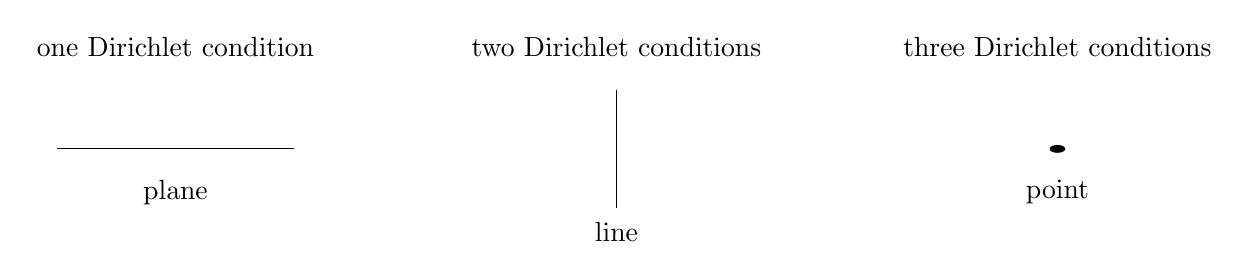
\begin{tikzpicture}[x=2cm,y=1cm]
\node at (0,1.3) {one Dirichlet condition};
\draw (-0.75,0) -- (0.75,0);
\node at (0,-0.55) {plane};

\node at (2.8,1.3) {two Dirichlet conditions};
\draw (2.8,-0.75) -- (2.8,0.75);
\node at (2.8,-1.05) {line};

\node at (5.6,1.3) {three Dirichlet conditions};
\fill (5.6,0) circle (0.05);
\node at (5.6,-0.55) {point};
\end{tikzpicture}
\caption{The tabletop counting argument from the lecture. Each Dirichlet condition removes one independent direction of endpoint motion.}
\end{figure}

Repeated T-dualities on different compact directions therefore generate the familiar ladder
\begin{equation}
\mathrm{D}8,\ \mathrm{D}7,\ \mathrm{D}6,\ \dots,\ \mathrm{D}0.
\end{equation}
This is the clean mathematical conclusion worth keeping from the noisier stretch of the transcript. The space-filling endpoint should be handled cautiously. If no direction is fixed, then one simply has ordinary open-string theory with free endpoints; that is the space-filling case, but it is better here to separate it from the newly discovered ladder of lower-dimensional anchoring objects.

The lecture makes one more move before leaving the subject. The argument begins with compact directions, but if on one side of the duality a compact direction is shrunk to be arbitrarily small, then on the dual side it becomes arbitrarily large and effectively noncompact. In that way the conclusion is broadened: D-branes can extend along directions that are, for all practical purposes, noncompact as well.

\section{Physics on Branes: Gauge Fields, Color, and Monopoles}

Now the lecture spends the payoff it promised at the beginning. Once D-branes exist, what do they do?

Begin with a single brane. Open strings ending on it are confined to move on its worldvolume. Their joining and splitting look like particle processes, and at low energies, where one does not excite the internal vibrational modes of the strings, the resulting theory on the brane is simply a quantum field theory. In the lecture this is read as a QED-like situation: strings with both ends on the brane behave like photon-like excitations on the brane, while strings with only one end on the brane play the role of charged matter.

With several parallel branes, the bookkeeping becomes more interesting. The lecture names three of them Red, Green, and Blue. An oriented open string can begin on one brane and end on another, so it carries an ordered pair of labels. That is exactly the sort of structure one expects in a nonabelian gauge theory.

\begin{figure}[htbp]
\centering
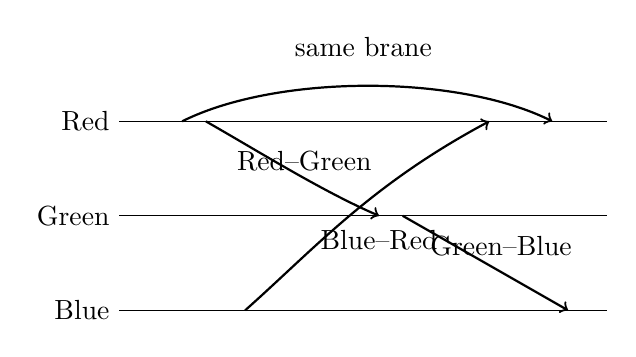
\begin{tikzpicture}[x=1cm,y=1cm]
\draw (0,2.4) -- (6.2,2.4);
\draw (0,1.2) -- (6.2,1.2);
\draw (0,0) -- (6.2,0);

\node[left] at (0,2.4) {Red};
\node[left] at (0,1.2) {Green};
\node[left] at (0,0) {Blue};

\draw[->,thick] (0.8,2.4) .. controls (2.0,3.0) and (4.3,3.0) .. (5.5,2.4);
\draw[->,thick] (1.1,2.4) .. controls (1.8,2.0) and (2.6,1.5) .. (3.3,1.2);
\draw[->,thick] (3.6,1.2) .. controls (4.3,0.8) and (5.0,0.4) .. (5.7,0);
\draw[->,thick] (1.6,0) .. controls (2.5,0.8) and (3.2,1.6) .. (4.7,2.4);

\node at (3.1,3.35) {same brane};
\node at (2.35,1.9) {Red--Green};
\node at (4.85,0.82) {Green--Blue};
\node at (3.3,0.9) {Blue--Red};
\end{tikzpicture}
\caption{Parallel branes with oriented open strings. Ordered endpoints furnish the pair of labels that mimic the gluon sector of a gauge theory living on the brane stack.}
\end{figure}

The lecture does not derive Yang--Mills theory from first principles. It follows the string processes instead. If a Red--Green string meets a Green--Blue string with compatible orientation, the relevant endpoints can join and produce a Red--Blue string. These are exactly the kinds of combinatorial rules one associates with nonabelian gauge bosons. At the same schematic level, one color-singlet combination can detach from the stack and is not part of the stable gluon sector, which is why the lecture remarks that one finds eight gluons rather than nine naive color-pair states.

Quarks are represented differently. A quark has one color label, not a color and an anticolor. In this brane language that means a string with only one end attached to the color stack; the other end extends elsewhere, to a distant brane or effectively off to infinity. A quark and an antiquark can annihilate when their compatible ends meet. Two quarks cannot.

With one brane the resulting worldvolume theory is abelian and QED-like. With several parallel branes the theory becomes nonabelian and QCD-like, at least in the lecture's schematic and supersymmetric sense. The important point is historical and structural: none of this was put in at the beginning. It is what the mathematics of open strings on D-branes naturally builds.

The last step is the magnetic one. The theory contains not only the ordinary fundamental strings but also D-strings, which are heavier one-dimensional D-branes. A D-string can end on a D3-brane. If an ordinary string endpoint on a D3-brane behaves like an electric charge, then the endpoint of a D-string behaves as its magnetic dual:
\begin{equation}
\text{D-string ending on a D3-brane}
\quad\longrightarrow\quad
\text{magnetic monopole}.
\end{equation}
Because D-strings are much heavier than fundamental strings, the corresponding monopoles are much heavier than the electric charges. The lecture does not attempt a full derivation of monopole dynamics; it uses the example to show how naturally electric and magnetic sectors are mirrored once D-branes are in place.

The lecture ends by stepping back. These structures were not invented in a single stroke. Over decades, string theorists kept reading the mathematics more carefully, and the mathematics kept insisting on the same conclusion. A theory that began life as a theory of hadrons became a theory of quantum gravity, and then, through T-duality and D-branes, looped back into a powerful tool for studying gauge theory.

\section{Summary}

The lecture unfolds in a precise sequence. We begin with a compact direction and closed oriented strings. That gives us two sectors, momentum and winding, with characteristic energies
\begin{equation}
E_{\text{mom}} \sim \frac{n}{r},
\qquad
E_{\text{wind}} \sim w\,r.
\end{equation}
Comparing the small-\(r\) and large-\(r\) regimes suggests the exchange
\begin{equation}
n\leftrightarrow w,
\qquad
r\leftrightarrow \frac{1}{r}.
\end{equation}
Then the lecture sharpens the statement by writing
\begin{equation}
P_y \propto \int d\sigma\,\frac{\partial y}{\partial \tau},
\qquad
W=\frac{1}{r}\int d\sigma\,\frac{\partial y}{\partial \sigma},
\end{equation}
so that T-duality becomes the exchange of \(\partial_\tau y\) with \(\partial_\sigma y\), together with an exchange of the spacetime fields that couple to momentum and winding.

Once the same idea is applied to open strings, Neumann boundary conditions in the compact direction become Dirichlet ones. Free endpoints become fixed endpoints. That is the moment at which D-branes are forced into the theory. From there the lecture moves outward: D\(p\)-branes of varying dimension, gauge theories on their worldvolumes, color labels from stacks of parallel branes, and magnetic monopoles from D-strings ending on D3-branes. T-duality is therefore not an isolated symmetry. It is one of the routes by which string theory discovers its own deeper ontology.